The \textit{Analyser} class in charge of manages all the phase in the pipeline, in other words, it sends to each module the required input in order to obtain is output. Besides, as it has been explained in Section \ref{section:typomod} where the typographic correction module was presented, it asks the user the necessary information for the purpose of detecting and correcting, if it is required, the found typographic errors. In addition to it, as we can see in Figure \ref{fig:umlanalyser}, this class is able to store information in the database and extract it through the \textit{SessionTypoError} class.

\begin{figure}[h]
	\centering%
	\centerline{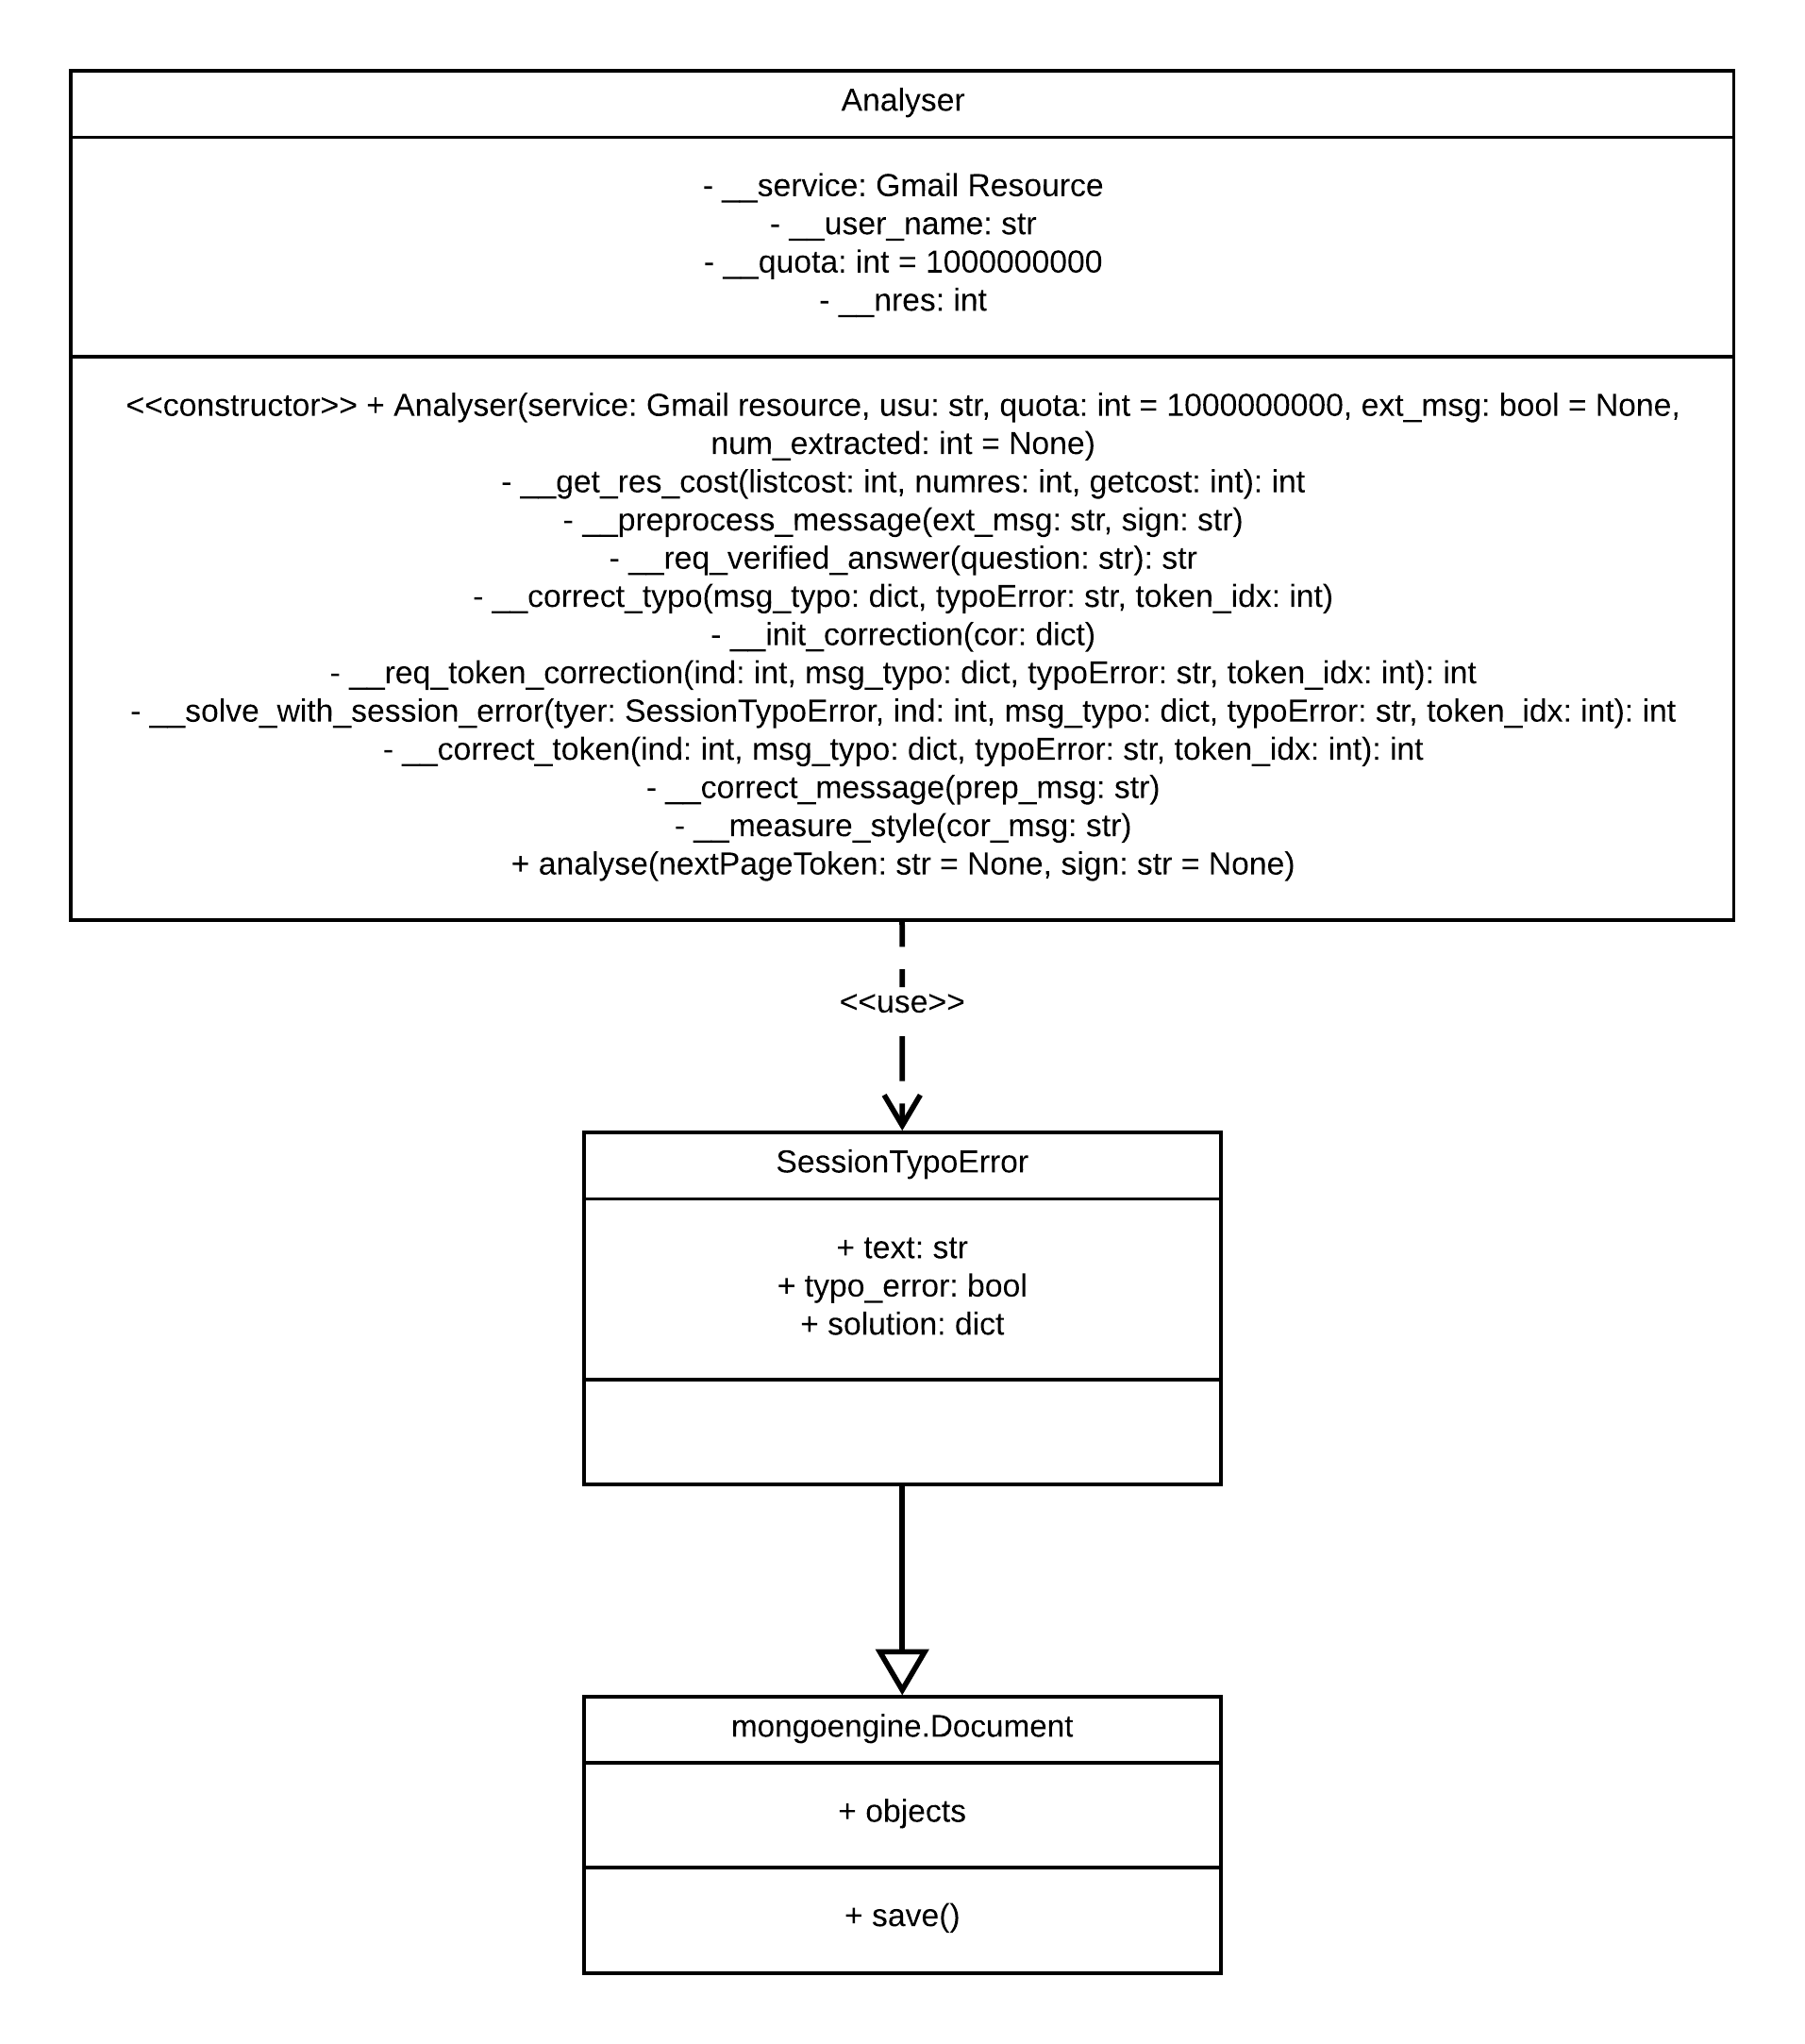
\includegraphics[width=0.6\paperwidth]{Imagenes/Bitmap/analyserUML.png}}%
	\caption{UML class diagram of the Analyser}%
	\label{fig:umlanalyser}
\end{figure}

The \textit{Analyser}'s class constructor has an special interest in this system, due to it chooses the type of extraction that is going to be executed: a message extraction or a thread extraction.